\section{Программная реализация}

\subsection{Структура пакетов}

\begin{figure}[!h]
\begin{center}
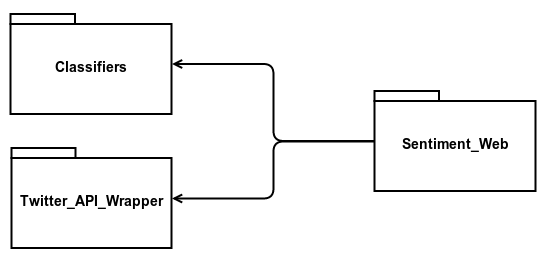
\includegraphics[scale=0.6, clip]{../resources/uml/packages.png}
\caption{Диаграмма пакетов}
\label{gr:packages}
\end{center}
\end{figure} 

Весь проект реализован с использованием языка программирования Python. Программная реализация состоит из трёх частей:
\begin{enumerate}
\item 
Пакет Classifiers содержит классы и функции для работы с
алгоритмами классификации, для выбора признаков,
перекрёстной проверки, а также для работы с корпусами данных.

\item 
Пакет Twitter\_API\_Wrapper содержит класс-обёртку для 
доступа Twitter API. Использует библиотеку python-oauth2.

\item 
Веб-приложение Sentiment\_WEB служит для поиска
мнений в социальной сети Twitter. 
\end{enumerate}

\subsection{Пакет Сlassifiers}

\subsubsection{Классификаторы}

Все классификаторы наследуются от базового класса ClassifierBase. 
Он имеет ссылки на экземпляры подклассов PreprocessorBase (предобработчики)
и FeatureExtractorBase (выделители признаков и выборщики признаков).
Это удобно, так как для сохранения классификатора на
диск (и для последующей загрузки) достаточно сериализовать 
один объект (сериализация осуществляется с помощью
стандартной библиотеки pickle).

В классе ClassifierBase определены следующие методы:
\begin{description}

\item[learn(documents, labels)] \hfill \\
Процедура обучения.
Принимает на вход массив документов обучающей выборки
и массив соответствующих документам классов 
(классами могут быть как строки, так и числа).
Определяется в наследниках.

\item[classify\_one(document)] \hfill \\
Функция классификации одного документа.
Принимает на вход документ (строку), возвращает класс,
предсказанный в соответствии с моделью.
Возвращает класс с максимальным значением
функции get\_conditional\_probability(document, class).

\item[classify\_batch(documents)] \hfill \\
Функция классификации множества документов.
Принимает на вход массив строк, возвращает массив классов.

\item[get\_conditional\_probability(document, class)] \hfill \\
Возвращает вероятность того, что документ принадлежит классу в соответствии с параметрами модели. Определяется в наследниках.

\item[get\_encoded\_labels(labels)] \hfill \\
Кодирует классы обучающей выборки в диапазон числами
от $0$ до $n-1$ ($n$ --- число уникальных классов).

\end{description}

\vspace{0.7cm}

В классе ClassifierBase определены следующие поля:
\begin{description}

\item[preprocessor] \hfill \\
Предобработчик нормализует документ. 

\item[feature\_extractor] \hfill \\
Выделитель признаков преобразует строку в признаковый вектор).

\item[class\_index] \hfill \\
Ассоциативный массив. Ключ --- оригинальный класс,
значение --- индекс от 0 до $n-1$.

\item[classes] \hfill \\
Массив уникальных классов.

\end{description}

\begin{figure}[!h]
\begin{center}
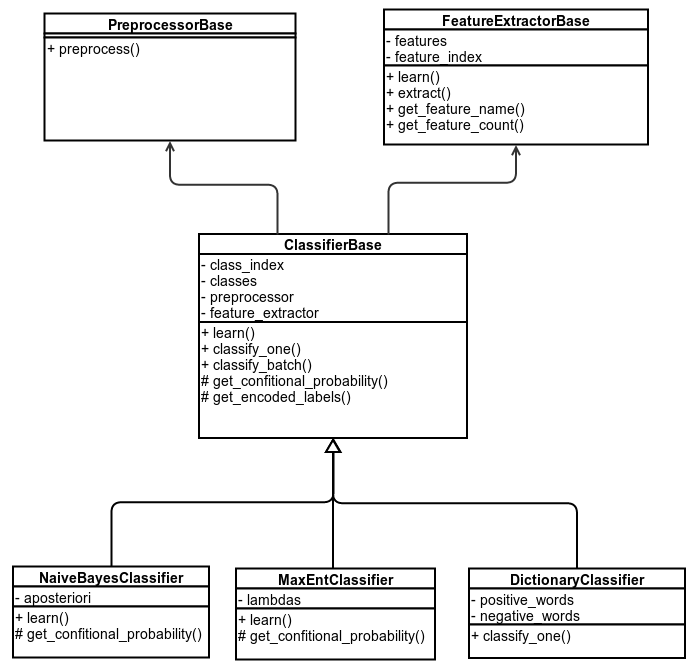
\includegraphics[scale=0.6, clip]{../resources/uml/classifiers_classes.png}
\caption{Диаграмма классов классификаторов}
\label{gr:classifiers}
\end{center}
\end{figure} 

\clearpage{}

\subsubsection{Выделители признаков}

Классификаторы работают с векторным представлением документа. 
Подклассы класса FeatureExtractorBase преобразовывают
текстовый документ в признаковый вектор (массив).

В нём определены следующие методы:
\begin{description}

\item[learn(documents, labels)] \hfill \\
Процедура обучения. Определяется в потомках.

\item[extract(document)] \hfill \\
Функция извлечения признаков. Принимает на вход строку,
возвращает признаковый вектор (массив).

\item[get\_feature\_count()] \hfill \\
Возвращает размер признакового вектора.

\end{description}

Выбор признаков осуществляется с помощью подкласса FeatureSelectorBase, который является декоратором FeatureExtractorBase. Таким образом, очень просто
добавить или убрать отбор признаков (классификатор
не знает, с чем он работает).

Извлечение n-грамм осуществляется с помощью
подкласса NgrammFeatureExtractor. В конструкторе ему передаётся массив требуемых n (можно использовать 1-граммы, 2-граммы и т.д. вместе или по-отдельности).

Подклассы NgrammFeatureExtractorBoolean и NgrammFeatureExtractorCount отличаются способом
определения веса у признаков.

\begin{figure}[!h]
\begin{center}
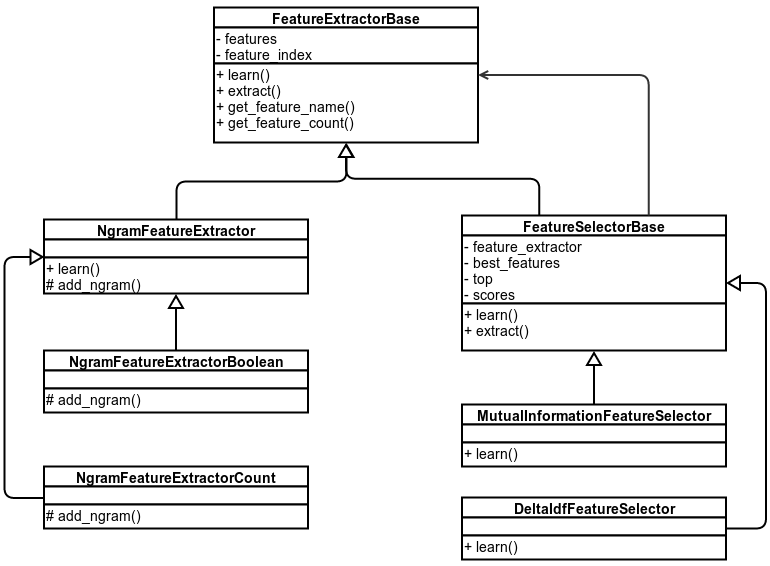
\includegraphics[scale=0.6, clip]{../resources/uml/feature_extractors_classes.png}
\caption{Диаграмма классов для выделителей признаков}
\label{gr:extractors}
\end{center}
\end{figure}

\clearpage{}

\subsubsection{Предобработчики}

Предобработчики выполняют нормализацию текста.

Во всех подклассах PreprocessorBase определён метод {\bf preprocess}, который получает на вход строку, применяет
к ней нормализующее действие, и возвращает нормализованную строку.

Для возможности гибкого изменения порядка нормализации
все атомарные действия реализованны отдельными классами,
которые объединяются с помощью компоновщика
CombinedPreprocessor.

\begin{figure}[!h]
\begin{center}
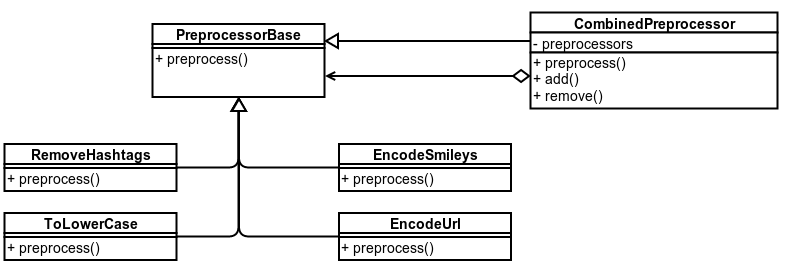
\includegraphics[scale=0.6, clip]{../resources/uml/preprocessor_classes.png}
\caption{Диаграмма классов для предобработчиков}
\label{gr:preprocessors}
\end{center}
\end{figure} 

\clearpage{}

\subsection{Пакет Twitter\_API\_Wrapper}
\begin{figure}[!h]
\begin{center}
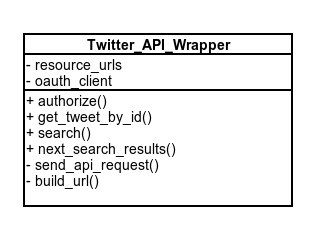
\includegraphics[scale=0.6, clip]{../resources/uml/twitter_classes.png}
\caption{Диаграмма классов клиента для Twitter}
\label{gr:preprocessors}
\end{center}
\end{figure} 

\subsection{Веб-приложение}
Веб-приложение было разработано при помощи веб-фреймворка Django.
Интерфейс разработан с помощи css-фреймворка ZURB Foundation.

На главной странице пользователь может ввести название
сущности, интересующей его. 
\begin{figure}[!ht]
\begin{center}
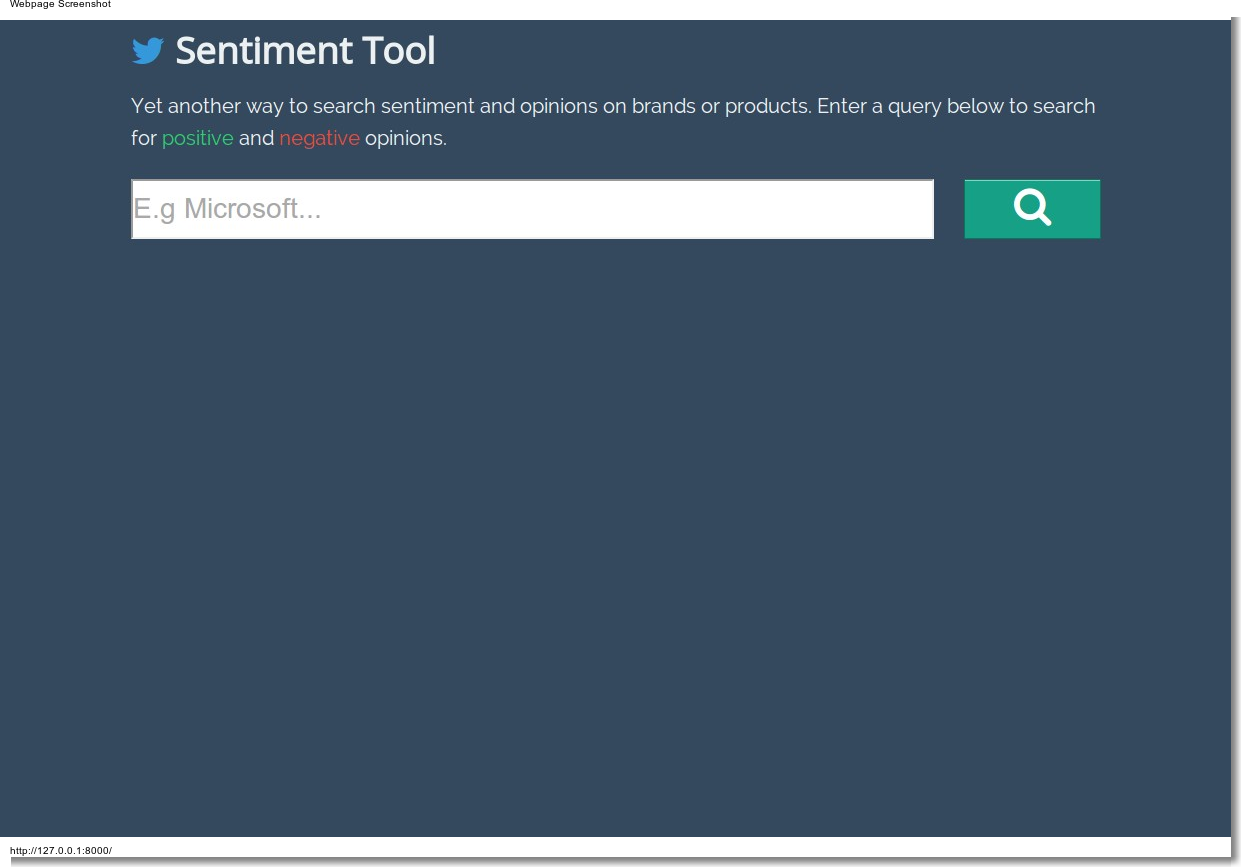
\includegraphics[scale=0.4, trim=20mm 60mm 20mm 10mm, clip]{../resources/screens/main.png}
\caption{Главная страница приложения}
\label{gr:mainpage}
\end{center}
\end{figure} 


После того, как пользователь кликнул на кнопку поиска, происходит ajax-запрос
к серверу. Сервер возвращает уже классифицированные сообщения в 
формате JSON. По умолчанию показываются последние 400 сообщений.

\begin{figure}[!ht]
\begin{center}
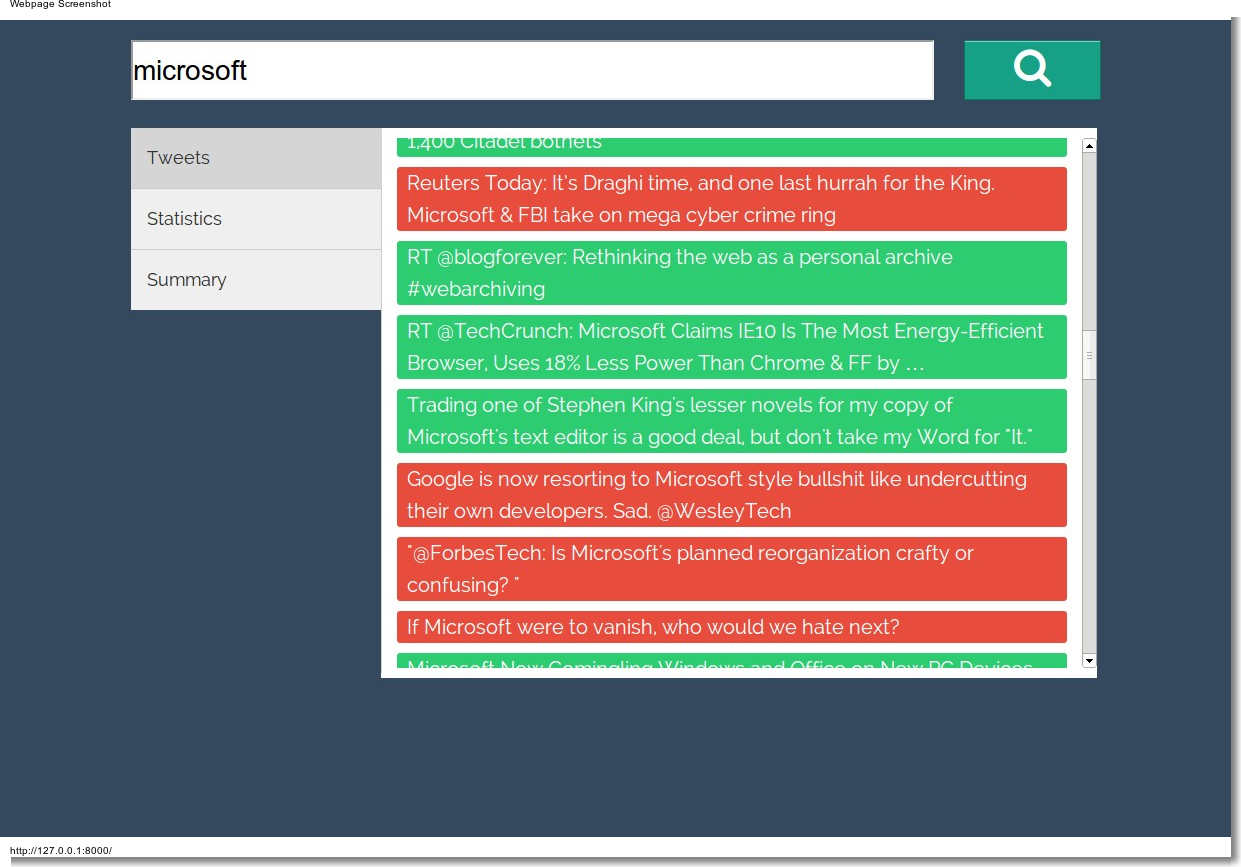
\includegraphics[scale=0.4, trim=20mm 60mm 20mm 10mm, clip]{../resources/screens/tweets.png}
\caption{Вкладка сообщений. Сообщения, имеющие отрицательную тональность подсвечены красным, положительную --- зелёным, нейтральную --- тёмно-синим.}
\label{gr:messages}
\end{center}
\end{figure} 

На вкладке ``Statistics'' (статистика) отображается количество сообщений каждой категории,
а также круговая диаграмма для того, чтобы быстро оценить общее мнение
об объекте поиска.
\begin{figure}[!ht]
\begin{center}
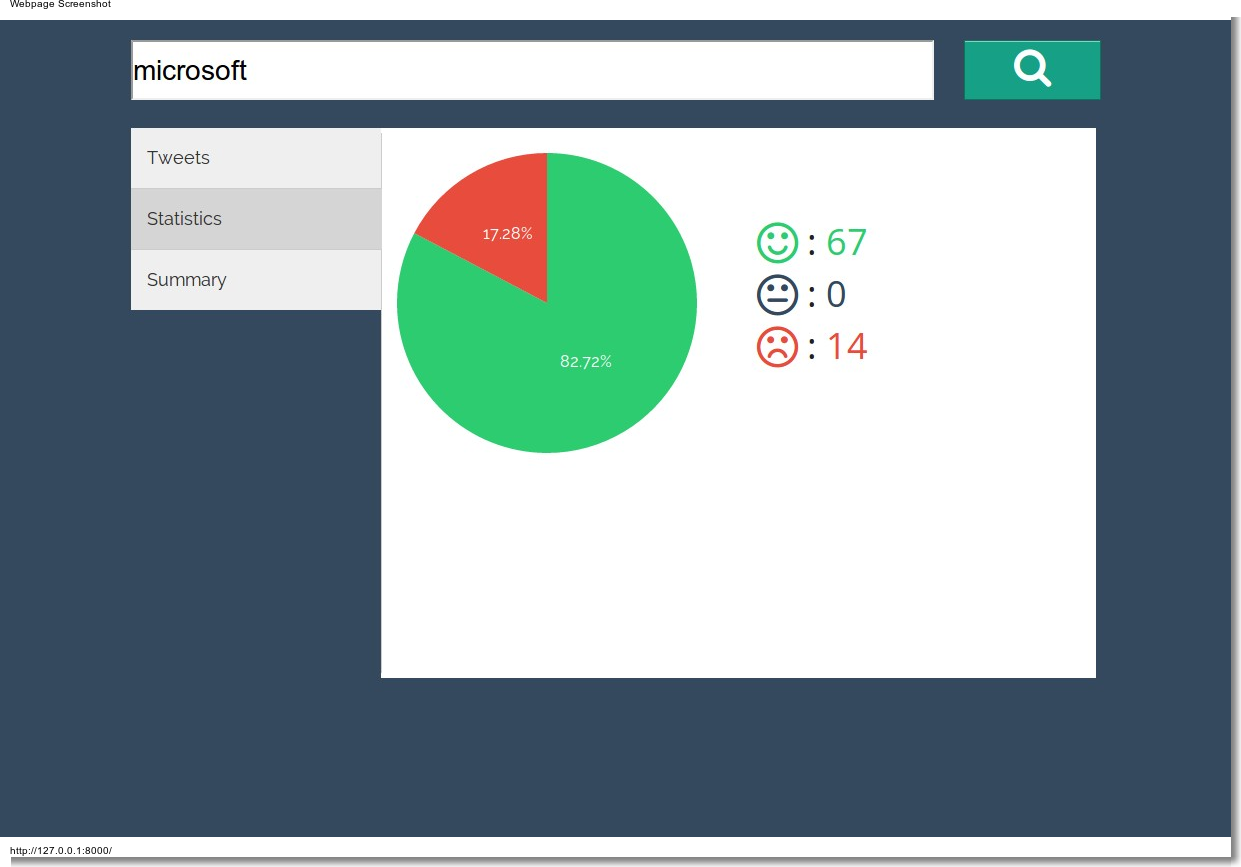
\includegraphics[scale=0.4, trim=20mm 60mm 20mm 10mm, clip]{../resources/screens/statistics.png}
\caption{Вкладка статистики}
\label{gr:stats}
\end{center}
\end{figure} 


На вкладке ``Summary'' (сводка) отображаются два облака слов --- положительное 
(популярные слова, употребляющиеся в позитивном контексте) и отрицательное.
Размер слова пропорционален логарифму частоты употребления.
\begin{figure}[!ht]
\begin{center}
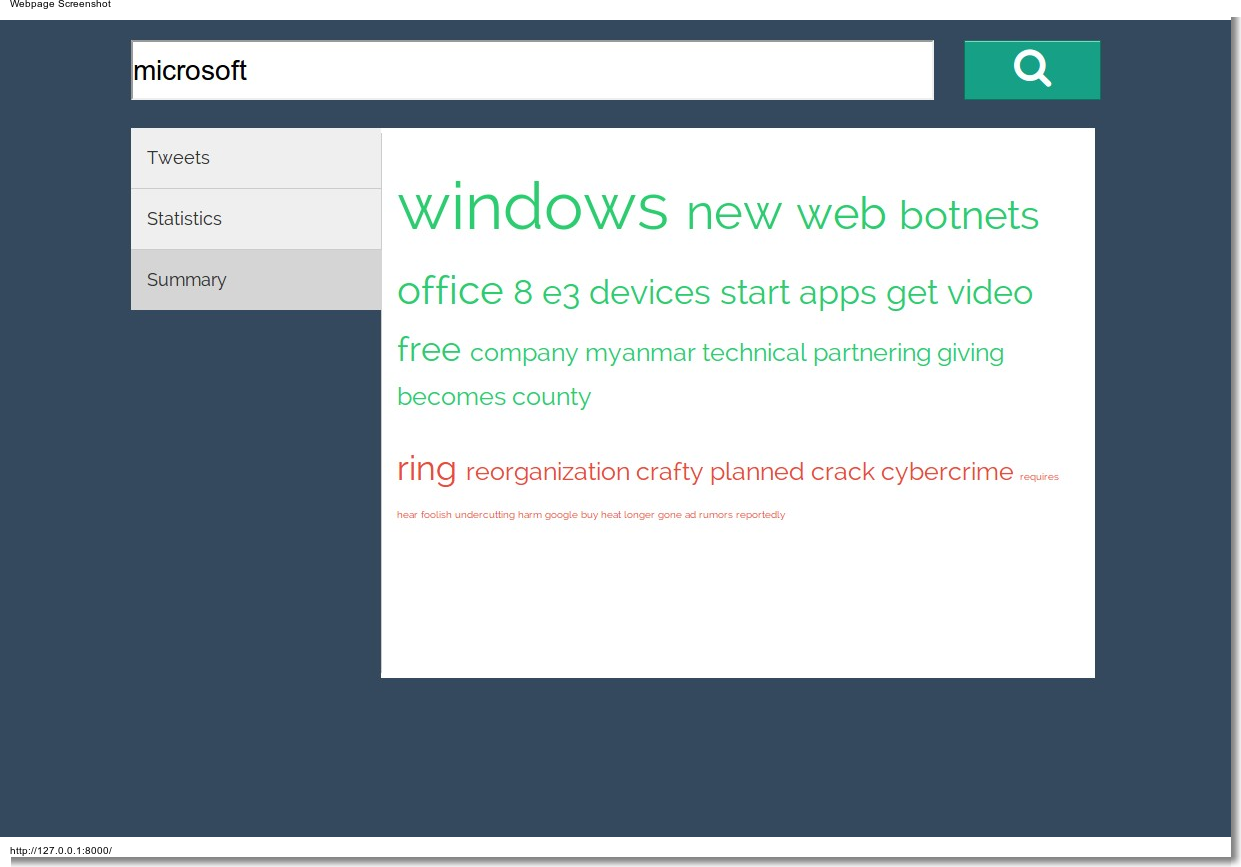
\includegraphics[scale=0.4, trim=20mm 60mm 20mm 10mm, clip]{../resources/screens/summary.png}
\caption{Вкладка сводки}
\label{gr:summary}
\end{center}
\end{figure} 

\clearpage{}